\chapter{Control System}
\label{ch:control_system}

The control system is one of the most important parts in the quadrotor's operation. In this research, we implemented a nonlinear attitude control system based on a dynamic model of the quadrotor. In this chapter, coordinate systems for the quadrotor's control are defined, the dynamic model of the quadrotor is introduced, and the control system is described.

\section{Control System Overview}
\label{sec:control_system_system_overview}

The overview of the control system is illustrated in Figure \ref{fig:bode}. First, the outer-loop controller receives desired position and desired attitude. Then, the outer-loop controller receives current state data from the sensors, and computes desired attitude and thrust corresponding to position errors of the quadrotor. The current position is estimated by synchronization of the internal accelerometer and barometer sensors, and other external sensors, such as a camera and a motion capture system. The inner-loop controller receives the quadrotor's attitude and angular velocity from the onboard gyroscope and magnetometer, and computes desired torque to control the attitude. The quadrotor's current attitude is measured by the internal magnetometer and angular velocity is measured by the internal gyroscope. Finally, the mixer, an open-loop motor controller, receives the desired thrust from the outer-loop controller and the desired torque from the inner-loop controller. Then, the mixer maps the desired thrust and torque into desired motor speeds, and estimates desired voltage of each motor.

\begin{figure}
    \centering
    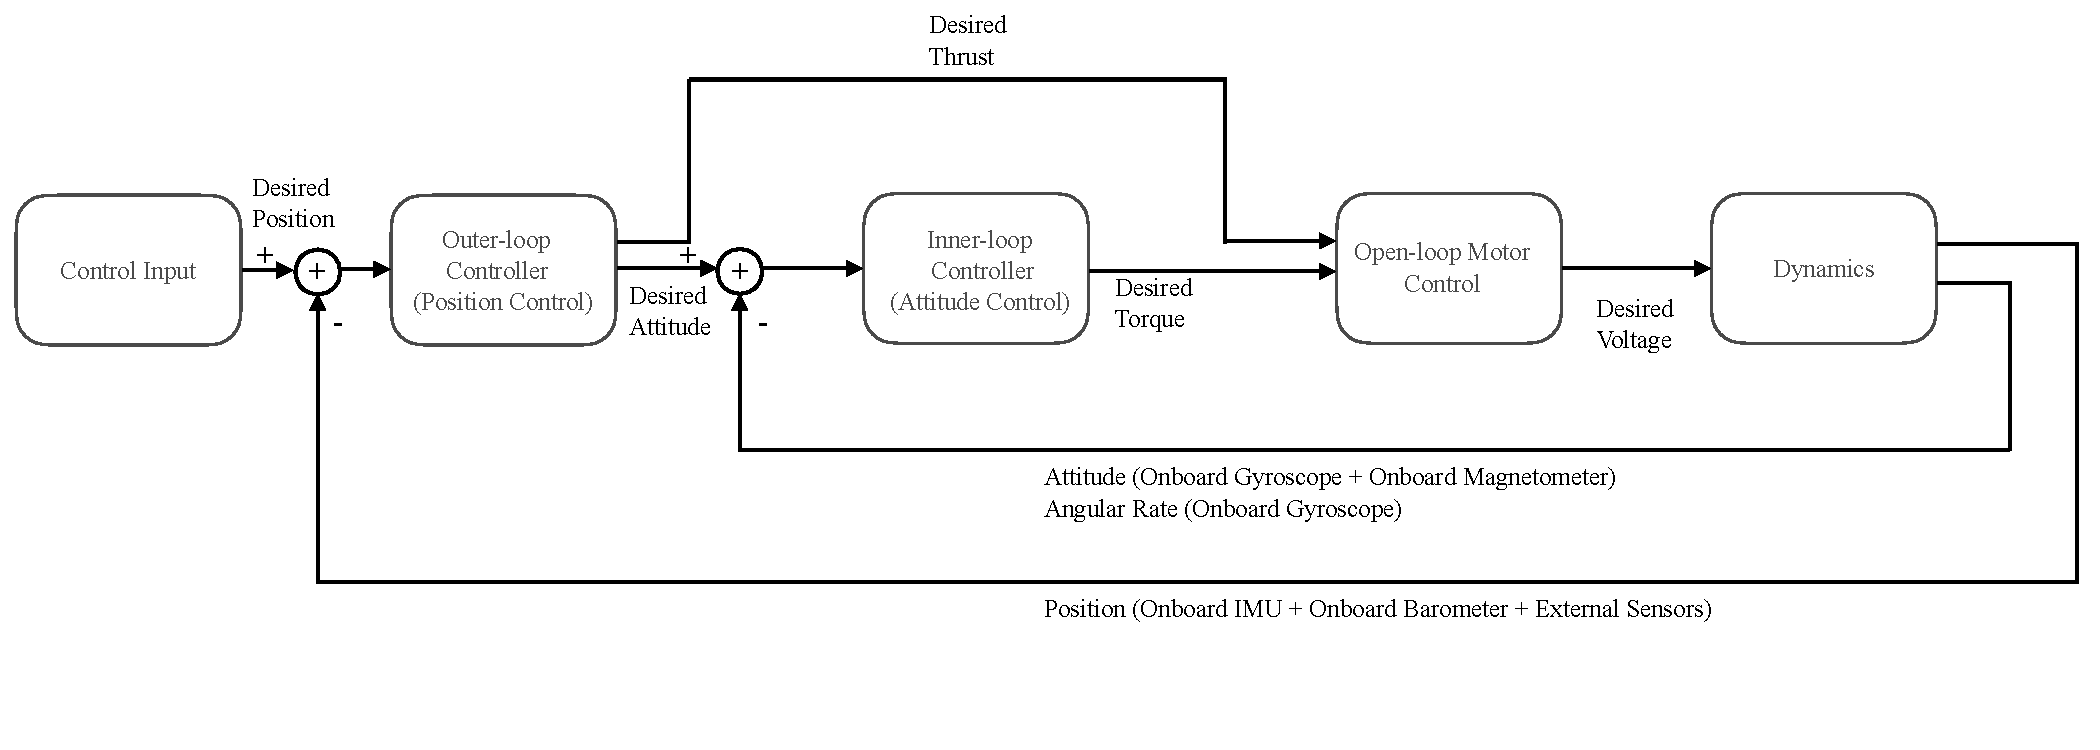
\includegraphics[width=1\textwidth]{graphics/bode_diagram.pdf}
    \caption{Illustration of the Control System.}
    \label{fig:bode}
\end{figure}

\section{Coordinate System}
\label{sec:coordinate_system}

In order to control the motion and state of the quadrotor, coordinate systems must be defined for the state and motion representation.\cite{intro_to_robotics} %john craig
First, a reference coordinate system must be defined to describe the orientation and position of the quadrotor. The reference coordinate system is called an "inertial coordinate system". Commonly, an inertial coordinate system is defined to be a Cartesian coordinate system that has its x, y-plane fixed on the ground. For convenience of control, the z-axis of the quadrotor is defined to face the ground. The origin can be arbitrarily set, but it is defined to be the initial position of the quadrotor in this research. 

In addition, it helps description of the quadrotor's motion to define a body-attached coordinate system since the onboard sensors of the quadrotor are fixed on the quadrotor's frame. In the quadrotor system, the body coordinate system follows the convention; the x, y-axises are defined to be parallel to the quadrotor's frame, and the z-axis is defined to be downward. The origin is set to be at the center of the autopilot controller, approximately at the center of mass.

\begin{figure}
    \centering
    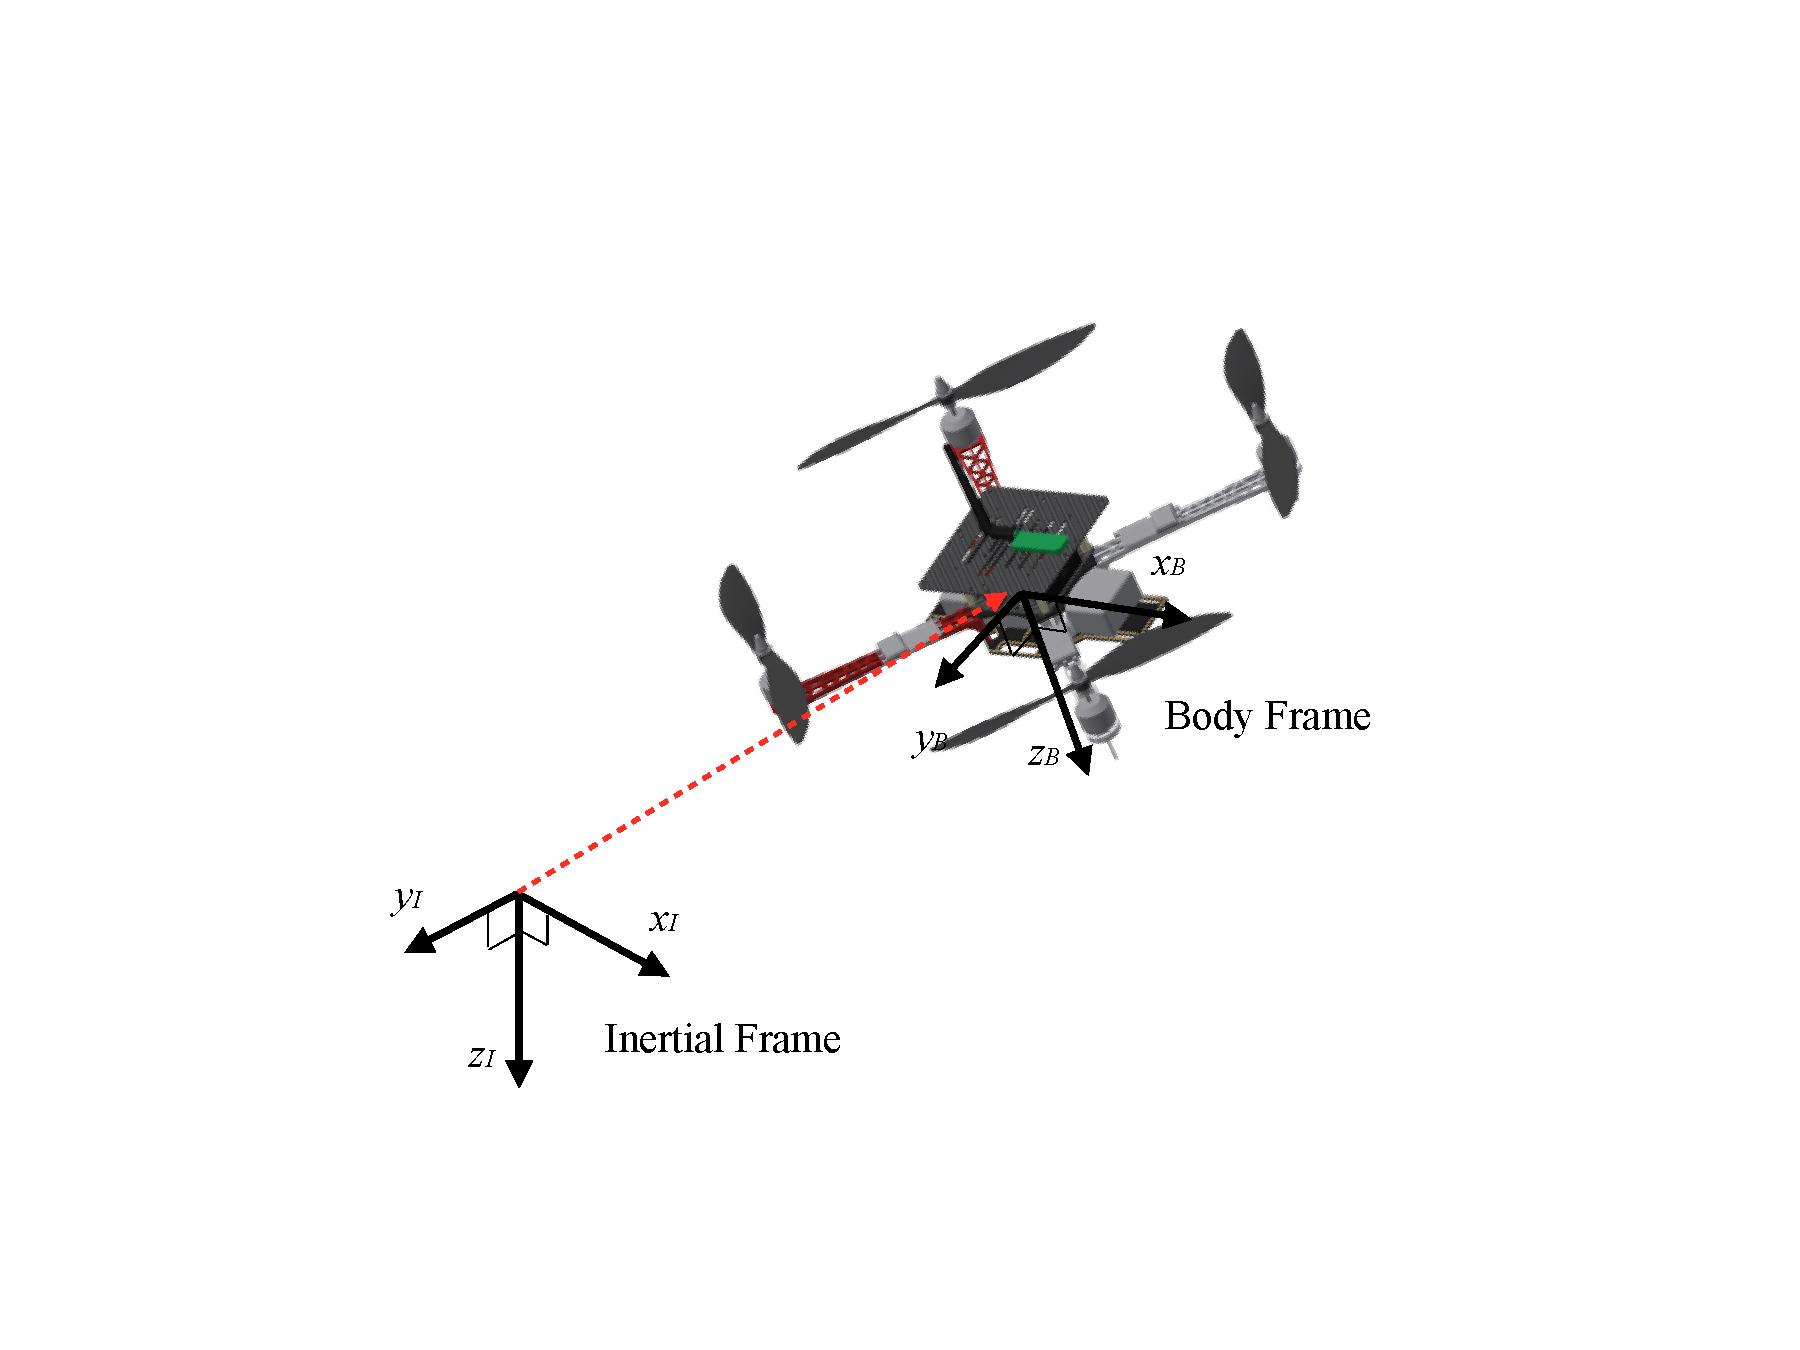
\includegraphics[width=0.8\textwidth]{graphics/coordinate.pdf}
    \caption{Illustration of the Inertial and Body Frames.}
    \label{fig:frame}
\end{figure}

Using the above coordinate systems, the quadrotor motion is represented completely. The mapping of the origin in the body frame into the inertial frame represents the quadrotor position. The orientation of the body frame is represented by multiple methods, such as the X-Y-Z fixed angles convention and the Z-Y-X Euler angles convention. In this research, the Z-Y-X Euler angles convention, also known as the Tait-Bryan angles convention, is used \cite{Diebel06}. In the Z-Y-X Euler angle convention, the mapping into the body frame starts with rotating about the z-axis by a yaw angle \(\psi\). Rotation of the y-axis by a pitch angle \(\theta\), and the z-axis by a roll angle \(\phi\) are followed in order. The transformation matrix of an orientation from the body frame into the inertial frame is given as,\\
\begin{equation}
\label{eq:transform_matrix}
\begin{aligned}
{^I _B}R
& = {R_{z, \psi}}  {R_{y, \theta}} {R_{x, \phi}}\\
& =
\begin{bmatrix}
\cos{\psi} & -\sin{\psi} & 0 \\
\sin{\psi} & \cos{\psi} & 0\\
0 & 0 & 1
\end{bmatrix}
\begin{bmatrix}
\cos{\theta} & 0& \sin{\theta} \\
0 & 1 & 0 \\
-\sin{\theta} & 0 & \cos{\theta}
\end{bmatrix}
\begin{bmatrix}
1 & 0 & 0\\
0& \cos{\phi} & -\sin{\phi} \\
0 & \sin{\phi} & \cos{\phi} \\
\end{bmatrix}\\
& =
\begin{bmatrix}
\cos{\theta} \cos{\psi} & \sin{\phi} \sin{\theta} \cos{\psi} - \cos{\phi}\sin{\psi} & \cos{\phi} \sin{\theta} \cos{\psi} + \sin{\phi} \sin{\psi}\\
\cos{\theta} \sin{\psi} & \sin{\phi} \sin{\theta} \sin{\psi} + \cos{\phi}\cos{\psi} & \cos{\phi} \sin{\theta} \sin{\psi} - \sin{\phi} \cos{\psi}\\
-\sin{\theta} &  \sin{\phi} \cos{\theta} & \cos{\phi} \cos{\theta}
\end{bmatrix}\\
\end{aligned}
\end{equation}
and the inverse transformation is given as,\\
\begin{equation}
\begin{aligned}
{^B _I}R
& = {{^B _I}R}^{-1}\\
& = {R_{x, \phi}}^{T}  {R_{y, \theta}}^{T} {R_{z, \psi}}^{T}\\
&=
\begin{bmatrix}
1 & 0 & 0\\
0& \cos{\phi} & \sin{\phi} \\
0 & - \sin{\phi} & \cos{\phi} \\
\end{bmatrix}
\begin{bmatrix}
\cos{\theta} & 0& - \sin{\theta} \\
0 & 1 & 0 \\
\sin{\theta} & 0 & \cos{\theta}
\end{bmatrix}
\begin{bmatrix}
\cos{\psi} & \sin{\psi} & 0 \\
-\sin{\psi} & \cos{\psi} & 0\\
0 & 0 & 1
\end{bmatrix}\\
& =
\begin{bmatrix}
  \cos{\theta} \cos{\psi}  &  \cos{\theta} \sin{\psi} & - \sin{\theta}  \\
\sin{\phi} \sin{\theta} \cos{\psi} - \cos{\phi} \sin{\psi} & \sin{\phi} \sin{\theta} \sin{\psi} + \cos{\phi} \cos{\psi} & \sin{\phi} \cos{\theta} \\
\cos{\phi} \sin{\theta} \cos{\psi}  +  \sin{\phi} \sin{\psi} & \cos{\phi} \sin{\theta} \sin{\psi}- \sin{\phi} \cos{\psi} & \cos{\phi}\cos{\theta}
\end{bmatrix}\\
\end{aligned}
\end{equation}

\section{Outer-Loop Controller}
\label{sec:outer_loop}

The outer-loop controller calculates desired attitude of the quadrotor, based on a given desired position and the quadrotor's current position. As a method of controlling the position of the quadrotor, PID control is applied. In this section, the outer-loop controller will be introduced. First, dynamics with respect to the quadrotor's position is described. Then, the position control of the quadrotor is stated.

\subsection{Dynamics Description}

A quadrotor is accelerated by thrust generated by its four rotors. Let \( {\boldsymbol F} = (\overline{X}, \overline{Y}, \overline{Z})\) be the quadrotor's thrust specified in the inertial frame. Then, the equation of motion is given as,
\begin{equation}
\label{eq:newton}
\begin{aligned}
m \ddot{{\boldsymbol{r}}} = \boldsymbol{F} + m \boldsymbol{g}\\
\end{aligned}
\end{equation}
where \(m\) is the mass of the quadrotor, \({\boldsymbol r} = (x, y, z)\) is the position of the quadrotor in the inertial frame, and \(\boldsymbol{g} = (0, 0, -g)\) is the gravitational acceleration.

Since the rotation axis of each rotor is fixed perpendicularly to the body, thrust can be generated only in the perpendicular direction of the body frame. Therefore, thrust can be computed by a rotation transformation from the body frame into the inertial frame. From equation (\ref{eq:transform_matrix}), thrust vector in the inertial frame is given as,
\begin{equation}
\begin{aligned}
{\boldsymbol F}
& = {^I_B}{R} 
\begin{bmatrix}
0\\
0\\
F
\end{bmatrix}\\
& =
\begin{bmatrix}
\cos{\theta} \cos{\psi} & \sin{\phi} \sin{\theta} \cos{\psi} - \cos{\phi}\sin{\psi} & \cos{\phi} \sin{\theta} \cos{\psi} + \sin{\phi} \sin{\psi}\\
\cos{\theta} \sin{\psi} & \sin{\phi} \sin{\theta} \sin{\psi} + \cos{\phi}\cos{\psi} & \cos{\phi} \sin{\theta} \sin{\psi} - \sin{\phi} \cos{\psi}\\
-\sin{\theta} &  \sin{\phi} \cos{\theta} & \cos{\phi} \cos{\theta}
\end{bmatrix}
\begin{bmatrix}
0\\
0\\
F
\end{bmatrix}\\
& =
F
\begin{bmatrix}
\cos{\phi} \sin{\theta} \cos{\psi} + \sin{\phi} \sin{\psi}\\
\cos{\phi} \sin{\theta} \sin{\psi} - \sin{\phi} \cos{\psi}\\
\cos{\phi} \cos{\theta}\\
\end{bmatrix}
\end{aligned}
\end{equation}
where \( F = \sqrt{{\overline{X}}^2 + {\overline{Y}}^2 + {\overline{Z}}^2}\) is the magnitude of the thrust, and \( {\boldsymbol \eta} = (\phi, \theta, \psi) \) is the attitude (roll, pitch, and yaw, respectively) of the quadrotor. Then, the thrust along each axis of the inertial frame is given as,
\begin{equation}
\label{eq:thrust_vector}
\begin{aligned}
{\overline X} &=  F (\cos{\phi} \sin{\theta} \cos{\psi} + \sin{\phi} \sin{\psi})\\
{\overline Y} &= F (\cos{\phi} \sin{\theta} \sin{\psi} - \sin{\phi} \cos{\psi})\\
{\overline Z} &=  F \cos{\phi} \cos{\theta}\\
\end{aligned}
\end{equation}
Therefore, from Equations (\ref{eq:newton}) and (\ref{eq:thrust_vector}), the acceleration of the quadrotor \({(\ddot{x}}, {\ddot{y}}, {\ddot{z}})\) is computed as,
\begin{equation}
\begin{aligned}
{{\ddot x} } & =  {F \over m} (\cos{\phi} \sin{\theta} \cos{\psi} + \sin{\phi} \sin{\psi})\\
{{\ddot y} } & =  {F \over m} (\cos{\phi} \sin{\theta} \sin{\psi} - \sin{\phi} \cos{\psi})\\
{{\ddot z} } & =  {F \over m} \cos{\phi} \cos{\theta} -g\\
\end{aligned}
\end{equation}

The sensors are fixed on the quadrotor, and therefore, it is necessary to formulate the relation of the quadrotor motion in the body frame and the inertial frame. Let \({\boldsymbol v}_B = (u, v, w)\) be the quadrotor's velocity in the body frame and \({\boldsymbol \omega} = (p, q, r)\) be the quadrotor's angular velocity. From the Coriolis effect, the equation of motion is given with respect to \( {\boldsymbol v}_B \) as the below equation \cite{randal08}.
\begin{equation}
\label{eq:newton_gravity}
\begin{aligned}
m \ddot{{\boldsymbol{r}}} = m (\dot{{\boldsymbol v}}_B + {\boldsymbol \omega} \times {\boldsymbol v}_B)\\
\end{aligned}
\end{equation}
Hence, from Equation (\ref{eq:newton}) the equation of the quadrotor's thrust \({\boldsymbol F}\) is written as,
\begin{equation}
\begin{aligned}
\boldsymbol{F} = m (\dot{{\boldsymbol v}}_B + {\boldsymbol \omega} \times {\boldsymbol v}_B- \boldsymbol{g})\\
\end{aligned}
\end{equation}

\subsection{Computation of Desired Velocity}
In order to control the quadrotor's position, the position controller sets desired velocity \({\boldsymbol v}_d = ({v_x}_d, {v_y}_d, {v_z}_d) \) in the inertial frame, with respect to the error of desired position \( {\boldsymbol{r}}_d = ({x_d} , {y_d} , {z_d} ) \) and observed position \( {{\boldsymbol{r}}}  = ({{x}} , {{y}} , {{z}} )\). The desired velocity is generated by P control. Desired control along each axis of the inertial frame is given as,
\begin{equation}
\begin{aligned}
{\boldsymbol v}_d = K_{pos} ( {\boldsymbol r}_d - {\boldsymbol r})\\
\end{aligned}
\end{equation}
where \( K_{pos} \) is a diagonal gain matrix of the controller. In order to prevent abnormal performance of the quadrotor, we set an upper limits of desired velocity. 

\subsection{Computation of Desired Thrust and Attitude}

In order to control the quadrotor's velocity, PID control can be applied to the motion of each axis in the inertial frame. A PID position control is given as the below equation \cite{Morgan16}\cite{giri}.
\begin{equation}
\label{eq:original_pid}
\begin{aligned}
{\overline X}_d & = m \left( \ddot{x}_d + {{K_P}_x}({x_d} - { x} ) + {{K_D}_x}({\dot {x}_d} -\dot{ x} ) + {{K }_I}_x \int_{t_0}^{t}({{x_d} - { x} }) dt \right) \\
{\overline Y}_d & = m \left( \ddot{y}_d + {{K_P}_y}({y_d} - { y} ) + {{K_D}_y}({\dot {y}_d} -\dot{ y} ) + {{K }_I}_y \int_{t_0}^{t}({{y_d} - { y} }) dt \right) \\
{\overline Z}_d & = m \left( g + \ddot{z}_d  + {{K_P}_z}({z_d} - { z} ) + {{K_D}_z}({\dot {z}_d} -\dot{ z} ) + {{K }_I}_z \int_{t_0}^{t}({{z_d} - { z} }) dt \right)\\
\end{aligned}
\end{equation}
\({{K_{P}}_x}\), \({{K_{P}}_y}\), \({{K_{P}}_z}\) are the gains of the proportional terms, \({{K_{D}}_x}\), \({{K_{D}}_y}\), \({{K_{D}}_z}\) are gains of the differential terms, and \({{K_{I}}_x}\), \({{K_{I}}_y}\), \({{K_{I}}_z}\) are gains of the integral terms.

The Pixhawk autopilot has been developed to support both indoor and outdoor flight. However, outdoor flight puts priority on velocity control, and considering outdoor environments, the control law of Equation (\ref{eq:original_pid}) may not work properly without precise position measurement. Therefore, a PID controller in terms of the quadrotor velocity is used alternatively in the autopilot system. The desired thrust of the alternative PID controller is given as,\\
\begin{equation}
\begin{aligned}
\ddot{x}  & = {1 \over m} \left( {{k_P}_x}({v_x}_d - \dot{ x} ) + {{k_D}_x}({\dot {v}_{x,d}} -\ddot{ x} ) + {{k_I }_x} \int_{t_0}^{t}({{v_x}_d - \dot{ x} }) dt \right)\\
\ddot{y}  & = {1 \over m} \left( {{k_P}_y}({v_y}_d - \dot{ y} ) + {{k_D}_y}({\dot {v}_{y,d}} -\ddot{ y} ) + {{k_I }_y} \int_{t_0}^{t}({{v_y}_d - \dot{ y} }) dt \right)\\
\ddot{z}  & = {1 \over m} \left( {{k_P}_z}({v_z}_d - \dot{ z} ) + {{k_D}_z}({\dot {v}_{z,d}} -\ddot{ z} ) + {{k_I }_z} \int_{t_0}^{t}({{v_z}_d - \dot{ z} }) dt \right)\\
\end{aligned}
\end{equation}
where \({{k_{P}}_x}\), \({{k_{P}}_y}\), \({{k_{P}}_z}\) are gains of the proportional terms, \({{k_{D}}_x}\), \({{k_{D}}_y}\), \({{k_{D}}_z}\) are gains of the differential terms, and \({{k_{I}}_x}\), \({{k_{I}}_y}\), \({{k_{I}}_z}\) are gains of the integral terms. Then, from Equation (\ref{eq:newton}), the desired thrust \({\overline X}_d, {\overline Y}_d, {\overline Z}_d \) can be computed as,
\begin{equation}
\label{eq:desired_thrust_vector}
\begin{aligned}
{\overline X}_d & = {{k_P}_x}({v_x}_d - \dot{ x} ) + {{k_D}_x}({\dot {v_x}_d} -\ddot{ x} ) + {{k_I }_x} \int_{t_0}^{t}({{v_x}_d - \dot{ x} }) dt\\
{\overline Y}_d & = {{k_P}_y}({v_y}_d - \dot{ y} ) + {{k_D}_y}({\dot {v_y}_d} -\ddot{ y} ) + {{k_I }_y} \int_{t_0}^{t}({{v_y}_d - \dot{ y} }) dt\\
{\overline Z}_d & = m g + {{k_P}_z}({v_z}_d - \dot{ z} ) + {{k_D}_z}({\dot {v_z}_d} -\ddot{ z} ) + {{k_I }_z} \int_{t_0}^{t}({{v_z}_d - \dot{ z} }) dt\\
\end{aligned}
\end{equation}

In this research, Equation (\ref{eq:desired_thrust_vector}) is used for outer-loop control, but the control law of Equation of (\ref{eq:original_pid}) is more appropriate for indoor flight with the values of \((\dot{x}_d, \dot{ y}_d, \dot{z}_d)\) and \((\ddot{x}_d, \ddot{ y}_d, \ddot{z}_d)\). In the control of Equation (\ref{eq:desired_thrust_vector}), the gains of differential terms are set small so that the effect of the differential terms is comparatively ignorable. Since the desired velocity is set proportionally with the error of the quadrotor position, the control law becomes similar to PD control in terms of the quadrotor position.

As described above, the direction of the thrust is defined by the orientation of the quadrotor. From Equations (\ref{eq:thrust_vector}), desired roll \(\phi_d\), pitch \(\theta_d\), and yaw \(\psi_d\) are computed as,
\begin{equation}
\label{eq:desired_attitude}
\begin{aligned}
\phi_d = \arcsin {{{{\overline X}_d} \sin{\psi_d} - {{\overline Y}_d} \cos{\psi_d}} \over {F_d}}\\
\theta_d = \arctan {{{{\overline X}_d} \cos{\psi_d} + {{\overline Y}_d} \sin{\psi_d}} \over {{\overline Z}_d}}\\
\end{aligned}
\end{equation}
Also, the magnitude of desired thrust \(F_d\) is given as,\\
\begin{equation}
\begin{aligned}
F_d & = | {\boldsymbol F}_d | \\
& =  \sqrt{{{\overline X}_d}^2 + {{\overline Y}_d}^2 + {{\overline Z}_d}^2}\\
\end{aligned}
\end{equation}
%This implies that with any given yaw angle, the position of the quadrotor is controllable. Therefore, yaw angle is also controllable while holding the quadrotor's position.
\( {{\overline X}_d} \), \({{\overline Y}_d}\), and \({{\overline Z}_d}\) are computed from Equation (\ref{eq:desired_thrust_vector}). Therefore, we can find that the desired roll \(\phi_d\) and pitch \(\theta_d\) are determined by the given desired yaw \(\psi_d\). 


\section{Inner-Loop Controller}
\label{sec:inner_loop}

The outer-loop controller computes desired attitude of the quadrotor based on position control. The inner-loop controller computes the torque required to control the quadrotor's attitude. PID control is often used as a method of attitude control. However, in this research, a more advanced control is applied for the inner-loop. In this section, a nonlinear inner-loop controller will be introduced. Firstly, dynamics with regard to the quadrotor's attitude is described. Then, a process of computing desired angular rate and torque of the quadrotor is explained. Finally, a proof of the controller's stability is stated.

\subsection{Dynamics Description}
Let \(\boldsymbol u = (u_p, u_q, u_r)\) be the torque in the body frame. Then, from the effect of rotation, the equation of moment is given with respect with the quadrotor angular velocity \({\boldsymbol \omega} = (p, q, r)\) as,\\
\begin{equation}
\label{eq:rotation}
\begin{aligned}
\boldsymbol{u} = {d \over dt}({J {\boldsymbol \omega}}) = J {\dot {\boldsymbol \omega}} -\text{Skew} (J {\boldsymbol \omega}) {\boldsymbol \omega}\\
\end{aligned}
\end{equation}
where \(J\) is the inertia matrix of the quadrotor \cite{Bolandi13}. \(\text{Skew} ({\boldsymbol a}) \) is a skew-symmetric matrix, defined as, \\
\begin{equation}
\begin{aligned}
\text{Skew} ({\boldsymbol a}) = 
\begin{bmatrix}
0 & - a_3 & a_2\\
a_3 & 0 & - a_1\\
-a_2 & a_1 & 0
\end{bmatrix}\\
\end{aligned}
\end{equation}
By considering the symmetry of the quadrotor along each axis of body frame, the diagonal elements \(J_{xx}\), \(J_{yy}\), \(J_{zz}\) are much greater than the other elements and, the non-diagonal elements are negligible. Therefore, the inertia matrix \(J\) is approximated as a positive diagonal matrix. \\
\begin{equation}
\begin{aligned}
J & \approx 
\begin{bmatrix}
J_{xx} & 0 & 0 \\
0 & J_{yy} & 0 \\
0 & 0 & J_{zz}
\end{bmatrix}
\end{aligned}
\end{equation}

Since the quadrotor attitude \({\boldsymbol \eta} = (\phi, \theta, \psi) \) is on the body frame, there is a relation between the angular velocity \({\boldsymbol \omega} = (p, q, r) \) and the derivative \( \dot{{\boldsymbol \eta}} = (\dot\phi, \dot\theta, \dot\psi)\) of the attitude, given by, \\
\begin{equation}
\begin{aligned}
\begin{bmatrix}
p\\
q\\
r
\end{bmatrix}
& =
\begin{bmatrix}
{\dot \phi} \\
0 \\
0
\end{bmatrix}
+ {R_{x, \phi}}^{T} \left(
\begin{bmatrix}
0 \\
{\dot \theta} \\
0
\end{bmatrix}
+ {R_{y, \theta}}^{T}
\begin{bmatrix}
0 \\
0 \\
{\dot \psi} 
\end{bmatrix}
\right) \\
& =
\begin{bmatrix}
{\dot \phi} \\
0 \\
0
\end{bmatrix}
+ 
\begin{bmatrix}
1 & 0    & 0 \\
0 & \cos{\phi}	& \sin{\phi} \\
0 & - \sin{\phi} 	& \cos{\phi}
\end{bmatrix}
\left(
\begin{bmatrix}
0 \\
{\dot \theta} \\
0
\end{bmatrix}
+
\begin{bmatrix}
\cos{\theta}	& 0    & - \sin{\theta}\\
0			& 1    & 0 \\
\sin{\theta}	&0	 & \cos{\theta}
\end{bmatrix}
\begin{bmatrix}
0 \\
0 \\
{\dot \psi} 
\end{bmatrix}
\right) \\
& = 
\begin{bmatrix}
1 	& 0    		& -\sin{\theta}\\
0 	& \cos{\phi}	& \sin{\phi} \cos{\theta} \\
0	& - \sin{\phi}	& \cos{\phi} \cos{\theta}
\end{bmatrix}
\begin{bmatrix}
{\dot \phi}\\
{\dot \theta} \\
{\dot \psi}
\end{bmatrix}\\
\end{aligned}
\end{equation}
Define a transform matrix \(Z\) from the body frame into the inertial frame with respect to the quadrotor attitude \({\boldsymbol \eta}\) as,\\
\begin{equation}
\begin{aligned}
Z = Z({\boldsymbol \eta}) = 
\begin{bmatrix}
1 	& 0    		& - \sin{\theta}\\
0 	& \cos{\phi}	& \sin{\phi} \cos{\theta} \\
0	& - \sin{\phi}	& \cos{\phi} \cos{\theta}
\end{bmatrix} ^{-1}
=
\begin{bmatrix}
1 & \sin{\phi} \tan{\theta}    & \cos{\phi} \tan{\theta}\\
0 & \cos{\phi}                     & - \sin{\phi} \\
0 & \sin{\phi} \sec{\theta} & \cos{\phi} \sec{\theta}
\end{bmatrix}\\
\end{aligned}
\end{equation}
Then, from the transformation of coordinate systems, the derivative of the attitude \(\dot{\boldsymbol \eta}\) can be written with respect to \({\boldsymbol \eta}\) and \(\dot{\boldsymbol \omega}\) as, \\
\begin{equation}
\label{eq:z_omega}
\begin{aligned}
{\dot {\boldsymbol \eta}} = Z {\boldsymbol \omega}\\
\end{aligned}
\end{equation}
Since the transformation matrix \(Z\) always has an inverse matrix regardless of the quadrotor attitude \({\boldsymbol \eta}\), the inverse form of the above equation is also satisfied. Therefore, the angular velocity is represented with the derivative of the attitude \(\dot{\boldsymbol \eta}\) and the transform matrix \(Z\), as the below equation.\\
\begin{equation}
\begin{aligned}
\label{eq:z_inv_eta}
{\boldsymbol \omega} = Z^{-1}{\dot {\boldsymbol \eta}} \\
\end{aligned}
\end{equation}


\subsection{Computation of Derivative of the Desired Attitude}
\label{subsec:desired_attitude}
The inner-loop controller receives desired attitude \( {\boldsymbol \eta}_d = (\phi_d, \theta_d, \psi_d) \) from the outer-loop controller, and desired angular velocity \({\boldsymbol \omega}_d\) is computed from it. From Equation (\ref{eq:z_omega}), the desired angular velocity is given from the controller as, \\
\begin{equation}
\begin{aligned}
{\boldsymbol \omega}_d = Z^{-1}{\dot {\boldsymbol \eta}_d} \\
\end{aligned}
\end{equation}
With the value of the desired attitude \( {\boldsymbol \eta}_d  \), there are multiple methods to compute the derivative of the desired attitude \({\dot {\boldsymbol \eta}_d}\).

First, \({\dot {\boldsymbol \eta}_d} = (\dot{\phi_d},\dot{ \theta_d}, \dot{\psi_d})\) is computed by direct differentiation of the desired attitude \({\dot {\boldsymbol \eta}}\) defined in Equation (\ref{eq:desired_attitude}). From Equation (\ref{eq:desired_attitude}), \({\dot {\boldsymbol \eta}_d}\) is computed as,
\begin{equation}
\begin{aligned}
\dot{\phi}_d & = {1 \over {\sqrt{1 - {c_1}^2}}} \left( c_2 \dot{\psi} + {\sin{\psi} \over F_d} \dot{{\overline X}}_d - {\cos{\psi} \over F_d} \dot{{\overline X}}_d  - {{c_1 \dot{F}_d} \over {{F_d}^2}} \right)\\
\dot{\theta}_d & = {1 \over {1 + {c_2}^2}} \left( - c_1 \dot{\psi} + {\cos{\psi} \over {{\overline Z}_d}} \dot{{\overline X}}_d + {\sin{\psi} \over {{\overline Z}}_d} \dot{{\overline X}}_d  +
- {{c_2 \dot{{\overline Z}}_d } \over {{{\overline Z}_d}^2}} \right)\\
\end{aligned}
\end{equation}
where \(c_1\) and \(c_2\) are defines as,
\begin{equation}
\begin{aligned}
c_1  = & {{{\overline X}_d} \sin{\psi} - {{\overline Y}_d} \cos{\psi}} \over {F_d}\\
c_2  = & {{{\overline X}_d} \cos{\psi} + {{\overline Y}_d} \sin{\psi}} \over {{\overline Z}_d}\\
\end{aligned}
\end{equation}
From geometric relation, the magnitude of the thrust, \(F_d = | {\boldsymbol F}_d | \), is written as,
\begin{equation}
\begin{aligned}
F_d = {{\overline Z}_d} \sec{\theta} \sec{\psi}
\end{aligned}
\end{equation}
Therefore, the roll rate \(\dot {\phi}_d\) is decoupled with \(F_d\), and represented with respect only with the attitude \(\boldsymbol \eta\) and the desired thrust \(({{\overline X}_d}, {{\overline Y}_d}, {{\overline Z}_d})\), as the below equation.
\begin{equation}
\begin{aligned}
\dot{\phi}_d & = {1 \over {\sqrt{1 - {c_1}^2}}} \left( c_2 \dot{\psi} + {\sin{\psi} \over F_d} \dot{{\overline X}}_d - {{\cos{\psi}} \over {F_d}} \dot{{{\overline X}}}_d  + {{c_1} \over {{F_d}^2}} \left({{\overline Z}_d} ( \dot{\phi} \sec{\phi} \tan{\phi}  + \dot{\theta} \sec{\theta} \tan{\theta} ) - \dot{{\overline Z}}_d \right) \right)\\
\end{aligned}
\end{equation}
Usually, yaw is controlled as constant, or yaw rate \(\dot{\psi}_d\) is given.

However, in the case that the quadrotor does not have precise measurement of its position, or the quadrotor's attitude is controlled manually, the above formulation may not be available. Therefore, an alternative computation method of desired angular velocity that uses a backward differentiation approximation can be applied. Numerically differentiated values usually have noise, and therefore, a low-pass filter is used to reduce noise. In discrete-time, let \(t_k\) be a discrete time and \({\Delta t}_k = t_k - t_{k-1}\) be a time step. Let \(u(t_k)\) be a raw value, and \(y(t_k)\) be a filtered value at time \(t_k\). Then, a first-order low-pass filter, also known as an exponentially weighted moving average filter, is given as the below equation, 
\begin{equation}
\label{eq:filter}
\begin{aligned}
y (t_{k}) = (1- a_k) u (t_{k}) - a_k y (t_{k-1})
\end{aligned}
\end{equation}
where the filter parameter \(a\) is defined with respect to the filter constant \(T_f\) as,
\begin{equation}
\begin{aligned}
a_k = {{{\Delta t}_k}\over{T_f + {\Delta t}_k}}
\end{aligned}
\end{equation}
In the above equation, the contribution of new input \(u (t_{k}) \) decreases and becomes less noisy as the filter constant \(T_f\) becomes greater. From the first-order differentiation approximation for the time derivative, raw derivative of the desired attitude is computed as the below equation.\\
\begin{equation}
\label{eq:numerical_desired_derivative}
\begin{aligned}
{\dot {\boldsymbol \eta}_{d,raw}}  (t_{k}) = {{{\boldsymbol \eta}_d (t_{k}) - {\boldsymbol \eta}_d (t_{k-1}) }\over {{\Delta t}_k}}
\end{aligned}
\end{equation}
From Equations (\ref{eq:filter}) and (\ref{eq:numerical_desired_derivative}), filtered derivative of the desired attitude is computed as the below equation.\\
\begin{equation}
\label{eq:filtered_desired_derivative}
\begin{aligned}
{\dot {\boldsymbol \eta}_d} (t_{k}) = (1- a_k ){\dot {\boldsymbol \eta}_{d,raw}} (t_{k})  - a_k {\dot {\boldsymbol \eta}_d} (t_{k-1})\\
\end{aligned}
\end{equation}
In the control system, Equation (\ref{eq:filtered_desired_derivative}) is used as derivative of the desired attitude.


\subsection{Computation of Desired Torque}

In this research, the nonlinear attitude control developed by Bandyopadhyay and Chung is used \cite{Bandyopadhyay16}. In the control law, previous to the computation of desired torque, it is necessary to define reference angular velocity. Let \( {\boldsymbol \eta} = (\phi, \theta, \psi) \) be actual attitude of the quadrotor. Define reference attitude \( {\dot {\boldsymbol \eta}_r}\) as, \\
\begin{equation}
\label{eq:eta_r}
\begin{aligned}
{\dot {\boldsymbol \eta}_r} & =  {\dot {\boldsymbol \eta}_d} + \Lambda( {\boldsymbol \eta}_d - {\boldsymbol \eta}) \\
\end{aligned}
\end{equation}
where \(\Lambda\) is a positive gain matrix as, \\
\begin{equation}
\begin{aligned}
\Lambda = 
\begin{bmatrix}
\lambda_{\phi}		& 0				& 0 \\
0				& \lambda_{\theta}	& 0 \\
0				& 0				& \lambda_{\psi}
\end{bmatrix}
> 0
\end{aligned}
\end{equation}
Reference angular velocity \({\boldsymbol \omega}_r \), and its derivative \( \dot{{\boldsymbol \omega}_r } \) are set as,\\
\begin{equation}
\begin{aligned}
{\boldsymbol \omega}_r & = Z^{-1} {\dot {\boldsymbol \eta}_d} + Z^{-1} \Lambda ({\boldsymbol \eta}_d - {\boldsymbol \eta})  \\
& = {\boldsymbol \omega}_d + Z^{-1} \Lambda ({\boldsymbol \eta}_d - {\boldsymbol \eta})\\
\end{aligned}
\end{equation}
\begin{equation}
\begin{aligned}
{\dot {\boldsymbol \omega}_r} & = {\dot {\boldsymbol \omega}_d} +  Z^{-1} \Lambda ({\dot {\boldsymbol \eta}_d} - \dot{\boldsymbol \eta}) -  Z^{-1} {\dot Z} Z^{-1}\Lambda ({{\boldsymbol \eta}_d} - {\boldsymbol \eta})\\
& = {\dot {\boldsymbol \omega}_d} + \Lambda \left( ({\boldsymbol \omega}_d - {\boldsymbol \omega}) -  Z^{-1} {\dot Z} Z^{-1} ({{\boldsymbol \eta}_d} - {\boldsymbol \eta}) \right)\\
\end{aligned}
\end{equation}
The reference angular velocity defined above includes both the desired angular velocity and a position error term. Therefore, it becomes a proportional feedback term to stabilize the quadrotor attitude when the error of the angular velocity is small. Since the matrix \(Z\) is an unitary matrix, \({\dot {\boldsymbol \omega}_r} \) can be simplified as,\\
\begin{equation}
\begin{aligned}
{\dot {\boldsymbol \omega}_r} = {\dot {\boldsymbol \omega}_d} + \Lambda ({\boldsymbol \omega}_d - {\boldsymbol \omega}) - Z^{-1} {\dot Z} Z^{-1} \Lambda ({{\boldsymbol \eta}_d} - {\boldsymbol \eta})
\end{aligned}
\end{equation}
For the implementation of the attitude control, we assume that \( \ddot{\boldsymbol \eta}_d = 0\), and this is equivalent to \({\dot {\boldsymbol \omega}_d} = 0\). The current attitude of the quadrotor \( {\boldsymbol \eta} \) and its derivative \({\dot {\boldsymbol \eta}}\) are estimated by filtered values of the internal magnetometer and the internal gyroscope.

According to the nonlinear attitude controller developed by Bandyopadhyay and Chung, the control law is given by the below equation \cite{Bandyopadhyay16}. \\
\begin{equation}
\label{eq:control_law}
\begin{aligned}
\boldsymbol{u} = J {\dot {\boldsymbol \omega}_r} - \text{Skew} (J {\boldsymbol \omega}) {\boldsymbol \omega}_r + K_{\omega} ({\boldsymbol \omega}_r - {\boldsymbol \omega}) 
\end{aligned}
\end{equation}
where is \(K_{\omega}\) a positive gain matrix, \\
\begin{equation}
\begin{aligned}
K_{\omega} = 
\begin{bmatrix}
{k_{\omega}}_p& 0	 			& 0 \\
0			& {k_{\omega}}_q	& 0 \\
0			& 0				& {k_{\omega}}_r
\end{bmatrix}
>0
\end{aligned}
\end{equation}

In order to prove stability of the nonlinear attitude controller, the Lyapunov method is used. From Equations (\ref{eq:z_omega}) and (\ref{eq:control_law}), the below equations are obtained.\\
\begin{equation}
\begin{aligned}
{\boldsymbol \omega}_r - {\boldsymbol \omega} & = {\boldsymbol \omega}_d -  {\boldsymbol \omega} + Z^{-1} \Lambda  ({\boldsymbol \eta}_d - {\boldsymbol \eta}) \\
\end{aligned}
\end{equation}
\begin{equation}
\begin{aligned}
(\dot{{\boldsymbol \eta}_d} - \dot{\boldsymbol \eta}) - Z({\boldsymbol \omega}_r - {\boldsymbol \omega}) + \Lambda  ({\boldsymbol \eta}_d - {\boldsymbol \eta}) = 0 \\
\end{aligned}
\end{equation}
From equations (\ref{eq:rotation}) and (\ref{eq:control_law}), the below equations can be obtained.\\
\begin{equation}
\begin{aligned}
 J {\dot {\boldsymbol \omega}} -\text{Skew} (J {\boldsymbol \omega}) {\boldsymbol \omega} = J {\dot {\boldsymbol \omega}_r} - {\text {Skew}}(J {\boldsymbol \omega}) {\boldsymbol \omega}_r + K_{\omega}  ({\boldsymbol \omega}_r - {\boldsymbol \omega})
\end{aligned}
\end{equation}
\begin{equation}
\begin{aligned}
J ({\dot {\boldsymbol \omega}_r} - {\dot {\boldsymbol \omega}}) + (K_{\omega} - {\text {Skew}}(J {\boldsymbol \omega})) ({\boldsymbol \omega}_r - {\boldsymbol \omega})
 = 0 \\
\end{aligned}
\end{equation}
Let \( {{\boldsymbol s}_1} = {\boldsymbol \omega}_r  - {\boldsymbol \omega} \) and \( {{\boldsymbol s}_2} = Z^{-1} ({\boldsymbol \eta}_d - {\boldsymbol \eta}) \). Then, the above equations can be written as, \\
% \begin{equation}
% \begin{aligned}
% \begin{bmatrix}
% J & 0 \\
% 0 & I
% \end{bmatrix}
% \begin{bmatrix}
% \dot{{\boldsymbol s}_1} \\
% \dot{{\boldsymbol s}_2}
% \end{bmatrix}
% +
% \begin{bmatrix}
% \text{Skew} (J {\boldsymbol \omega}) +  K_{\omega} & 0 \\
% -Z & \Lambda
% \end{bmatrix}
% \begin{bmatrix}
% {\boldsymbol s}_1 \\
% {\boldsymbol s}_2
% \end{bmatrix}
% =
% \begin{bmatrix}
% 0 \\
% 0
% \end{bmatrix}
% \end{aligned}
% \end{equation}
\color{blue} %%%%%%%%%%
\begin{equation}
\begin{aligned}
\begin{bmatrix}
J & 0 \\
0 & I
\end{bmatrix}
\begin{bmatrix}
\dot{{\boldsymbol s}_1} \\
\dot{{\boldsymbol s}_2}
\end{bmatrix}
+
\begin{bmatrix}
- \text{Skew} (J {\boldsymbol \omega}) +  K_{\omega} & 0 \\
-Z & \Lambda
\end{bmatrix}
\begin{bmatrix}
{\boldsymbol s}_1 \\
{\boldsymbol s}_2
\end{bmatrix}
=
\begin{bmatrix}
0 \\
0
\end{bmatrix}
\end{aligned}
\end{equation}
\color{black} %%%%%%%%%%
where \(I\) is the \(3 \times 3\) identity matrix. Define a Lyapunov function \( V\) as below, \\
\begin{equation}
\begin{aligned}
V({\boldsymbol s}_1, {\boldsymbol s}_2) = 
\begin{bmatrix}
{\boldsymbol s}_1 \\
{\boldsymbol s}_2
\end{bmatrix} ^{T}
\begin{bmatrix}
J & 0 \\
0 & I
\end{bmatrix}
\begin{bmatrix}
{{\boldsymbol s}_1} \\
{{\boldsymbol s}_2}
\end{bmatrix}
\end{aligned}
\end{equation}\\
Since the inertia matrix \(J\), and the identity matrix \( I\) are positive definite, the Lyapunov function \(V({\boldsymbol s}_1, {\boldsymbol s}_2) \) is positive, if \({\boldsymbol s}_1\), \({\boldsymbol s}_2\) are not zeros.
\begin{equation}
\begin{aligned}
V({\boldsymbol s}_1, {\boldsymbol s}_2) & =  {{\boldsymbol s}_1}^{T} J {\boldsymbol s}_1 + {{\boldsymbol s}_2}^{T} I {\boldsymbol s}_2  > 0 \\
\end{aligned} 
\end{equation}
Derivative \({\dot{V}({\boldsymbol s}_1, {\boldsymbol s}_2)}\) of the Lyapunov function is given below, and from the definition of \(K_{\omega}\) and \(\Lambda\), the derivative of the Lypunov function is negative definite, if \({\boldsymbol s}_1\), \({\boldsymbol s}_2\) are not zeros. \\ 
% \begin{equation}
% \begin{aligned}
% \dot{V}({\boldsymbol s}_1, {\boldsymbol s}_2) & = 
% \begin{bmatrix}
% {\boldsymbol s}_1 \\
% {\boldsymbol s}_2
% \end{bmatrix} ^{T}
% \begin{bmatrix}
% \dot{J} & 0 \\
% 0 & \dot{I}
% \end{bmatrix}
% \begin{bmatrix}
% {\boldsymbol s}_1 \\
% {\boldsymbol s}_2
% \end{bmatrix}
% + 2
% \begin{bmatrix}
% {\boldsymbol s}_1 \\
% {\boldsymbol s}_2
% \end{bmatrix} ^{T}
% \begin{bmatrix}
% J & 0 \\
% 0 & I
% \end{bmatrix}
% \begin{bmatrix}
% \dot{{\boldsymbol s}_1} \\
% \dot{{\boldsymbol s}_2}
% \end{bmatrix} \\
% & = 2
% \begin{bmatrix}
% {\boldsymbol s}_1 \\
% {\boldsymbol s}_2
% \end{bmatrix} ^{T}
% \begin{bmatrix}
% J & 0 \\
% 0 & I
% \end{bmatrix}
% \begin{bmatrix}
% {\boldsymbol s}_1 \\
% {\boldsymbol s}_2
% \end{bmatrix} \\
% & = 
% \begin{bmatrix}
% {\boldsymbol s}_1 \\
% {\boldsymbol s}_2
% \end{bmatrix} ^{T}
% \begin{bmatrix}
% 2 {\text {Skew}}(J {\boldsymbol \omega}) - 2K_{\omega} & 0 \\
% 2Z &  -2 \Lambda
% \end{bmatrix}
% \begin{bmatrix}
% {\boldsymbol s}_1 \\
% {\boldsymbol s}_2
% \end{bmatrix} \\
% & = 2  {{\boldsymbol{s}}_1}^{T} \text{Skew} (J {\boldsymbol \omega}) {\boldsymbol{s}}_1 - 2 {{\boldsymbol{s}}_1}^{T} K_{\omega} {\boldsymbol{s}}_1 -  2 {{\boldsymbol{s}}_2}^{T} \Lambda {\boldsymbol{s}}_2\\
% & =  - 2 {{\boldsymbol{s}}_1}^{T} K_{\omega} {\boldsymbol{s}}_1 -  2 {{\boldsymbol{s}}_2}^{T} \Lambda {\boldsymbol{s}}_2\\
% & < 0 \\
% \end{aligned}
% \end{equation} \\
% From the definition of \(K_{\omega}\) and \(\Lambda\), \(\dot{V} ({\boldsymbol s}_1, {\boldsymbol s}_2)\) is negative, if \({\boldsymbol s}_1\), \({\boldsymbol s}_2\) are not zeros.
% \begin{equation}
% \begin{aligned}
% \dot{V} ({\boldsymbol s}_1, {\boldsymbol s}_2) & =
% \begin{bmatrix}
% {\boldsymbol s}_1 \\
% {\boldsymbol s}_2
% \end{bmatrix} ^{T}
% \begin{bmatrix}
%  2 \text{Skew} (I Z^{-1} \dot{\boldsymbol \eta}) - 2K_{\omega} & 0 \\
% 2I &  -2 \Lambda
% \end{bmatrix}
% \begin{bmatrix}
% {\boldsymbol s}_1 \\
% {\boldsymbol s}_2
% \end{bmatrix} \\
% & = 2 {{\boldsymbol{s}}_1}^{T} \text{Skew} (I Z^{-1} \dot{\boldsymbol \eta}) {\boldsymbol{s}}_1 - 2 {{\boldsymbol{s}}_1}^{T} K_{\omega} {\boldsymbol{s}}_1 -  2 {{\boldsymbol{s}}_2}^{T} \Lambda {\boldsymbol{s}}_2 \\
% & =  - 2 {{\boldsymbol{s}}_1}^{T} K_{\omega} {\boldsymbol{s}}_1 -  2 {{\boldsymbol{s}}_2}^{T} \Lambda {\boldsymbol{s}}_2\\
% & < 0 \\
% \end{aligned}
% \end{equation}
\color{blue} %%%%%%%%%%
\begin{equation}
\begin{aligned}
\dot{V}({\boldsymbol s}_1, {\boldsymbol s}_2) & = 
\begin{bmatrix}
{\boldsymbol s}_1 \\
{\boldsymbol s}_2
\end{bmatrix} ^{T}
\begin{bmatrix}
\dot{J} & 0 \\
0 & \dot{I}
\end{bmatrix}
\begin{bmatrix}
{\boldsymbol s}_1 \\
{\boldsymbol s}_2
\end{bmatrix}
+ 2
\begin{bmatrix}
{\boldsymbol s}_1 \\
{\boldsymbol s}_2
\end{bmatrix} ^{T}
\begin{bmatrix}
J & 0 \\
0 & I
\end{bmatrix}
\begin{bmatrix}
\dot{\boldsymbol s}_1 \\
\dot{\boldsymbol s}_2
\end{bmatrix} \\
& = 
2
\begin{bmatrix}
{\boldsymbol s}_1 \\
{\boldsymbol s}_2
\end{bmatrix} ^{T}
\begin{bmatrix}
J & 0 \\
0 & I
\end{bmatrix}
\begin{bmatrix}
\dot{\boldsymbol s}_1 \\
\dot{\boldsymbol s}_2
\end{bmatrix} \\
& =
\begin{bmatrix}
{\boldsymbol s}_1 \\
{\boldsymbol s}_2
\end{bmatrix} ^{T}
\begin{bmatrix}
2 {\text {Skew}}(J {\boldsymbol \omega}) - 2K_{\omega} & 0 \\
2Z &  -2 \Lambda
\end{bmatrix}
\begin{bmatrix}
{\boldsymbol s}_1 \\
{\boldsymbol s}_2
\end{bmatrix}\\
& = 
\begin{bmatrix}
{\boldsymbol s}_1 \\
{\boldsymbol s}_2
\end{bmatrix} ^{T}
\begin{bmatrix}
- 2K_{\omega} & 0 \\
2Z &  -2 \Lambda
\end{bmatrix}
\begin{bmatrix}
{\boldsymbol s}_1 \\
{\boldsymbol s}_2
\end{bmatrix}\\
& =  - 2 {{\boldsymbol{s}'}_1}^{T} K_{\omega} {\boldsymbol{s}'}_1 - 2 {{\boldsymbol{s}'}_2}^{T} \Lambda {\boldsymbol{s}'}_2\\
& < 0 \\
\end{aligned}
\end{equation} \\
where \({\boldsymbol s'}_1 = U {\boldsymbol s}_1 \), \({\boldsymbol s'}_2 = U {\boldsymbol s}_2 \), and \(U\) is the unitary matrix such that
\begin{equation}
\begin{aligned}
U^{T}
\begin{bmatrix}
- 2K_{\omega} & 0 \\
2Z &  -2 \Lambda
\end{bmatrix}
U
=
\begin{bmatrix}
- 2K_{\omega} & 0 \\
0 &  -2 \Lambda
\end{bmatrix}\\
\end{aligned}
\end{equation}
\color{black} %%%%%%%%%%
Hence, by the Lyapunov 2nd method, the controller is globally asymptotic stable with an equilibrium point where \( {\boldsymbol s_1} =  0\), \( {\boldsymbol s_2} =  0\). Therefore, the quadrotor's attitude \({\boldsymbol \eta}\) and angular velocity \({\boldsymbol \omega}\) converge to \({\boldsymbol \eta}_d\) and \({\boldsymbol \omega}_d \), respectively.

Further, define \(c_1 =  \min(J_{xx}, J_{yy}, J_{zz}, 1) \) and \(c_2 =  \max(J_{xx}, J_{yy}, J_{zz}, 1) \), and then, the below condition of the Lyapunov function \({V} ({\boldsymbol s}_1, {\boldsymbol s}_2) \) is satisfied. Here, \({V} ({\boldsymbol s}_1, {\boldsymbol s}_2) \) is radially unbounded. \\
\begin{equation}
\begin{aligned}
\forall {\boldsymbol s}_1, {\boldsymbol s}_2 \neq {\boldsymbol 0}, \quad  c_2 (\|{{\boldsymbol s}_1}\|^2 +\|{{\boldsymbol s}_2}\|^2) > V({\boldsymbol s}_1, {\boldsymbol s}_2) & \approx  {{\boldsymbol s}_1}^{T} J {\boldsymbol s}_1 + {{\boldsymbol s}_2}^{T} I {\boldsymbol s}_2  >  c_1 (\|{{\boldsymbol s}_1}\|^2 +\|{{\boldsymbol s}_2}\|^2) > 0\\
\end{aligned}
\end{equation} 
Also, define \(c_3 = 2 \min(k_{\omega_p}, k_{\omega_q}, k_{\omega_r}, \lambda_{\phi}, \lambda_{\theta}, \lambda_{\psi}) \) and then, the below condition of \(\dot{V} ({\boldsymbol s}_1, {\boldsymbol s}_2) \) is satisfied.
\begin{equation}
\begin{aligned}
\forall {\boldsymbol s}_1, {\boldsymbol s}_2 \neq {\boldsymbol 0}, \quad \dot{V} ({\boldsymbol s}_1, {\boldsymbol s}_2) & \le - c_3 (\|{{\boldsymbol s}_1}\|^2 +\|{{\boldsymbol s}_2}\|^2) < 0
\end{aligned}
\end{equation} 
From the Lyapunov 1st method, the controller is globally exponentially stable as well without perturbation \cite{nonlinear_systems}. Hence it gives bounded errors that can be estimated with respect to bounded disturbance or modeling errors \cite{Bandyopadhyay16}.

\section{Motor Control}
\label{sec:motor_control}

As described in Section \ref{sec:inner_loop}, the desired torque of the quadrotor is computed by the inner-loop controller. The next step is to compute desired motor speed corresponding to the torque, and to control the motors. In the quadrotor system, the part that performs this step is called the "mixer". In this section, an advanced mixer for the quadrotor will be introduced. First, an aerodynamic model with respect to rotors is described, and a mapping method from attitude and thrust control into motor speed is explained. Then, dynamic model of a brushless DC motor for the quadrotor and its control are stated.

\subsection{Mapping Attitude and Thrust Control into Motor Speeds}

\begin{figure}
    \centering
    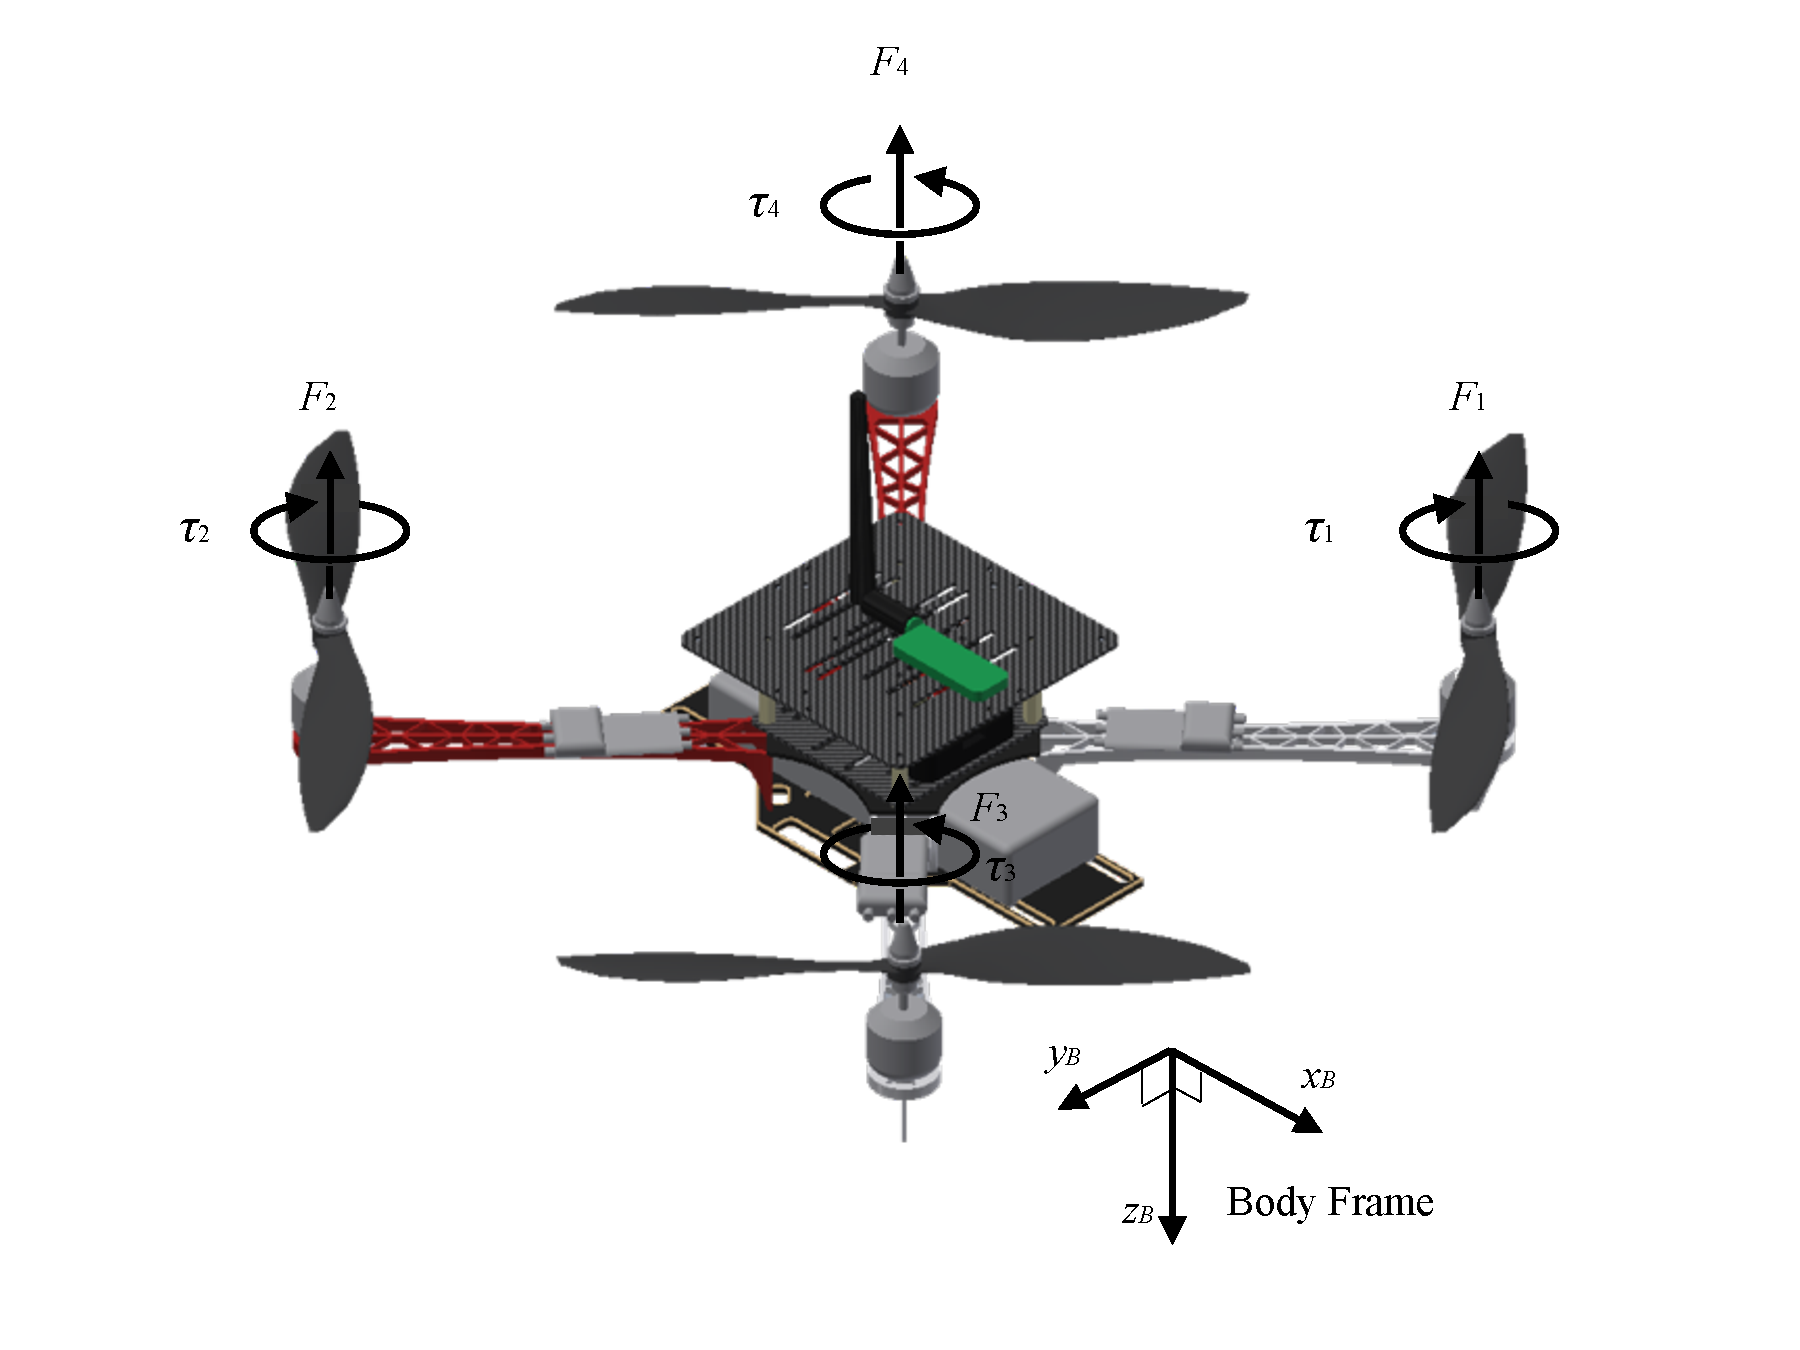
\includegraphics[width=0.8\textwidth]{graphics/mixer.pdf}
    \caption{Thrust and Torque Generated by Each Rotor}
    \label{fig:mixer}
\end{figure}

In the mixer, the magnitude of the desired thrust \(F_d\) from the outer-loop and the desired attitude control \({\boldsymbol \tau} = (\tau_{\phi}, \tau_{\theta}, \tau_{\psi})\) from the inner-loop are received. In order to map the attitude control and the desired thrust into motor speed \( {\boldsymbol n} = (n_1, n_2, n_3, n_4)\) , an aerodynamic model of the quadrotor can be applied.

It is known that the property of propeller is given with non-dimensional thrust coefficient \(C_T\) and power coefficient \(C_P\) as, \\
\begin{equation}
\begin{aligned}
C_T (n_i) ={ T \over { \rho {n_i}^2 D^4}}
\end{aligned}
\end{equation}
\begin{equation}
\begin{aligned}
C_P (n_i) = {P \over { \rho {n_i}^3 D^5}}
\end{aligned}
\end{equation}
where \(\rho\) is the density of air, \(D\) is the propeller's diameter, and \(T\), \(P\) are thrust and torque generated by a propeller, respectively \cite{airfoil2}. Here, \(C_T\) and \(C_P\) change according to rotation speed, and their curves are varied across different geometry of propellers and other conditions. Let \(F_i \) be the thrust force of each motor (\( i = 1, 2, 3, 4 \)) corresponding to its motor speed \( n_i\). With the experimental data of \(C_T\) and \(C_P\), thrust \( F_i\) and torque \(\tau_i\) generated by a motor according to its motor speed \( n_i\) are given as below,\\
\begin{equation}
\begin{aligned}
F_i = C_T (n_i) \rho {n_i}^2 D^4
\end{aligned}
\end{equation}
\begin{equation}
\begin{aligned}
\tau_i & = {P \over {2 \pi n_i}} \\ 
& = {C_P (n_i) \rho {n_i}^2 D^5 \over {2 \pi}}
\end{aligned}
\end{equation}

Since the quadrotor uses an X-shape frame in which the formation of the motors is a square, there is a linear relation as, \\
\begin{equation}
\begin{aligned}
F & = F_1 + F_2 + F_3 + F_4 \\
\tau_{\phi} & = {l \over {\sqrt{2}}} ( - F_1 + F_2 + F_3 - F_4)\\
\tau_{\theta} & = { l \over {\sqrt{2}}} (  F_1 - F_2 + F_3 - F_4)\\
\tau_{\psi} & =  \tau_1 + \tau_2 - \tau_3 - \tau_4
\end{aligned}
\end{equation}
where \(l\) to the length of the frame \cite{randal08}. We define an aerodynamic coefficient matrix \(B ({\boldsymbol n})\) as,
\begin{equation}
\begin{aligned}
B ({\boldsymbol n}) = 
\begin{bmatrix}
C_T (n_1)	& C_T (n_2)	& C_T (n_3)	& C_T (n_4)\\
- {l \over{\sqrt{2}}} C_T (n_1)		& {l \over{\sqrt{2}}} C_T (n_2)		& {l \over{\sqrt{2}}} C_T (n_3)	& - {l \over{\sqrt{2}}} C_T (n_4) \\
{l \over{\sqrt{2}}} C_T (n_1)		& - {l \over{\sqrt{2}}} C_T (n_2)		& {l \over{\sqrt{2}}} C_T (n_3)	& - {l \over{\sqrt{2}}} C_T (n_4) \\
{D \over{2\pi}} C_P (n_1)			& {D \over{2\pi}} C_P	 (n_2)		& - {D \over{2\pi}} C_P (n_3)	& - {D \over{2\pi}} C_P (n_4)
\end{bmatrix}
\end{aligned}
\end{equation}
Then, the above equation can be written as,\\
\begin{equation}
\label{eq:u_n}
\begin{aligned}
\begin{bmatrix}
F_d\\
u_p\\
u_q\\
u_r
\end{bmatrix}
= \rho D^4 B ({\boldsymbol n})
\begin{bmatrix}
{n_1}^2 \\
{n_2}^2 \\
{n_3}^2 \\
{n_4}^2
\end{bmatrix}
\end{aligned}
\end{equation}
With the above equation, motor speed \({\boldsymbol n} \) corresponding to the magnitude of the desired thrust \(F_d\) and the attitude control \({\boldsymbol \tau}\) can be computed as, \\
\begin{equation}
\label{eq:n_u}
\begin{aligned}
\begin{bmatrix}
{n_1}^2 \\
{n_2}^2 \\
{n_3}^2 \\
{n_4}^2
\end{bmatrix}
= {1 \over \rho D^4 }B^{-1} ({\boldsymbol n})
\begin{bmatrix}
F_d\\
u_p\\
u_q\\
u_r
\end{bmatrix}
\end{aligned}
\end{equation}


%%%%%%%%%%%%%%%%%%%%%%%%%%%%%%%%%%%%%%%%%%%%%%%%%%%%%%%%%%%%%%%%%%%%%%%%%%%%%%%%%%%%%%%%%%%%%%
\subsection{Approximation of the Aerodynamic Coefficient Matrix}
Since the coefficient matrix \( B ({\boldsymbol n}) \) is not independent from motor speed \(n_i\), it is difficult to compute a solution of Equation (\ref{eq:n_u}). To solve the problem, the linear approximation in terms of \(1 \over {n_i}^2\) as,\\
\begin{equation}
\label{eq:ct_approx}
\begin{aligned}
C_T ({n_i}) & = {C_T}_0 + {C_T}_1 {1 \over {n_i}^2} + O \left({1 \over {n_i}^4} \right) \\
& \approx {C_T}_0 + {C_T}_1 {1 \over {n_i}^2} \\
\end{aligned}
\end{equation}
\begin{equation}
\label{eq:cp_approx}
\begin{aligned}
C_P ({n_i}) & = {C_P}_0 + {C_P}_1 {1 \over {n_i}^2} + O \left({1 \over {n_i}^4} \right) \\
& \approx {C_P}_0 + {C_P}_1 {1 \over {n_i}^2}
\end{aligned}
\end{equation}
can be applied. Then, Equation (\ref{eq:u_n}) can be written as, \\
\begin{equation}
\begin{aligned}
\begin{bmatrix}
F_d\\
u_p\\
u_q\\
u_r
\end{bmatrix}
\approx \rho D^4 \left( B_0
\begin{bmatrix}
{n_1}^2 \\
{n_2}^2 \\
{n_3}^2 \\
{n_4}^2
\end{bmatrix}
+ B_1 
\begin{bmatrix}
1\\
1\\
1\\
1
\end{bmatrix} \right)
\end{aligned}
\end{equation}
where the approximation terms of \( B_0\), \(B_1\) of the matrix \(B ({\boldsymbol n}) \) are defined as,
\begin{equation}
\begin{aligned}
B_0 = 
\begin{bmatrix}
{C_T}_0	& {C_T}_0 	& {C_T}_0		& {C_T}_0 \\
- {l \over{\sqrt{2}}} {C_T}_0		& {l \over{\sqrt{2}}} {C_T}_0		& {l \over{\sqrt{2}}} {C_T}_0	& - {l \over{\sqrt{2}}} {C_T}_0 \\
{l \over{\sqrt{2}}} {C_T}_0		& - {l \over{\sqrt{2}}} {C_T}_0		& {l \over{\sqrt{2}}} {C_T}_0	& - {l \over{\sqrt{2}}} {C_T}_0 \\
{D \over{2\pi}} {C_P}_0			& {D \over{2\pi}} {C_P}_0		& - {D \over{2\pi}} {C_P}_0		& - {D \over{2\pi}} {C_P}_0
\end{bmatrix}
\end{aligned}
\end{equation}
\begin{equation}
\begin{aligned}
B_1 = 
\begin{bmatrix}
{C_T}_1	& {C_T}_1 	& {C_T}_1		& {C_T}_1 \\
- {l \over{\sqrt{2}}} {C_T}_1		& {l \over{\sqrt{2}}} {C_T}_1		& {l \over{\sqrt{2}}} {C_T}_1	& - {l \over{\sqrt{2}}} {C_T}_1 \\
{l \over{\sqrt{2}}} {C_T}_1		& - {l \over{\sqrt{2}}} {C_T}_1		& {l \over{\sqrt{2}}} {C_T}_1	& - {l \over{\sqrt{2}}} {C_T}_1 \\
{D \over{2\pi}} {C_P}_1			& {D \over{2\pi}} {C_P}_1		& - {D \over{2\pi}} {C_P}_1	& - {D \over{2\pi}} {C_P}_1
\end{bmatrix}
\end{aligned}
\end{equation}
Then, desired motor speeds \( \boldsymbol n\) are easily computed from the below equation,
\begin{equation}
\begin{aligned}
\begin{bmatrix}
{n_1}^2 \\
{n_2}^2 \\
{n_3}^2 \\
{n_4}^2
\end{bmatrix}
\approx
{B_0}^{-1}
\left(
{1 \over {\rho D^4}}
\begin{bmatrix}
F_d\\
u_p\\
u_q\\
u_r
\end{bmatrix}
- B_1
\begin{bmatrix}
1\\
1\\
1\\
1
\end{bmatrix}
\right)
\end{aligned}
\end{equation}

\begin{figure}
    \centering
    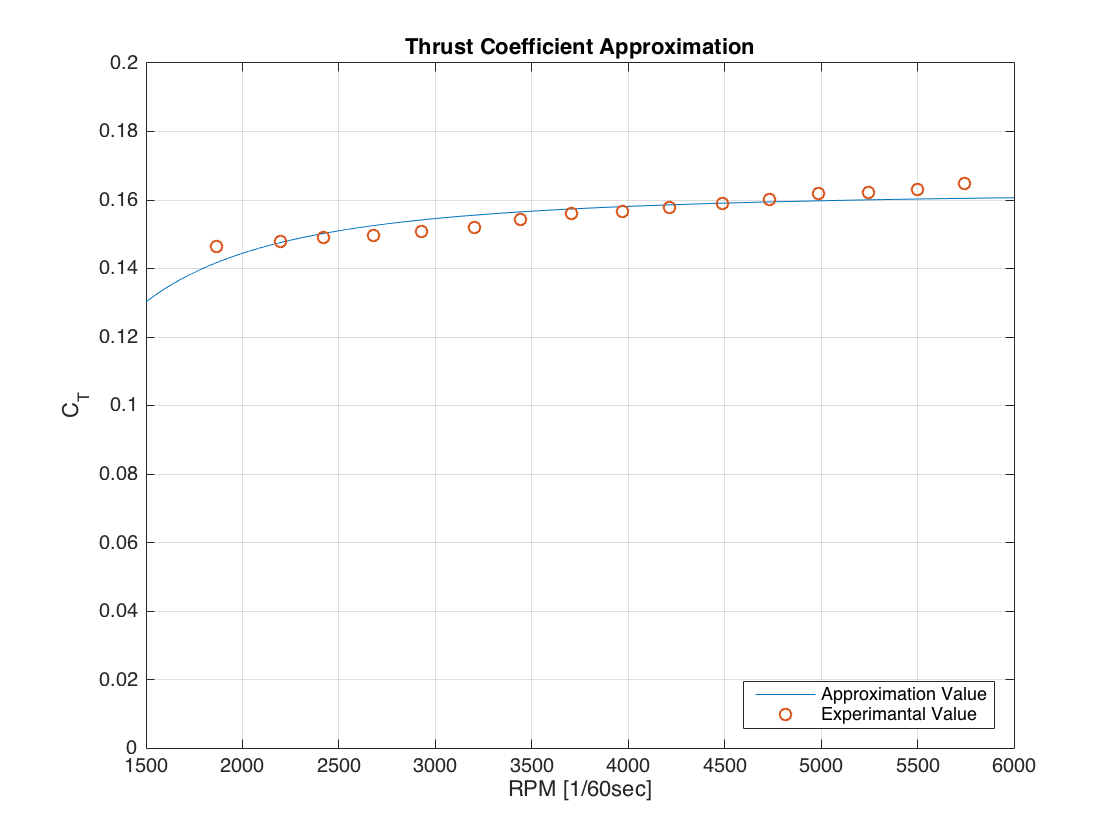
\includegraphics[width=0.8\textwidth]{graphics/Ct_fig.png}
    \caption{Comparison of experimental and approximated thrust coefficient}
    \label{fig:ct}
    
    \vspace{1cm}
    
    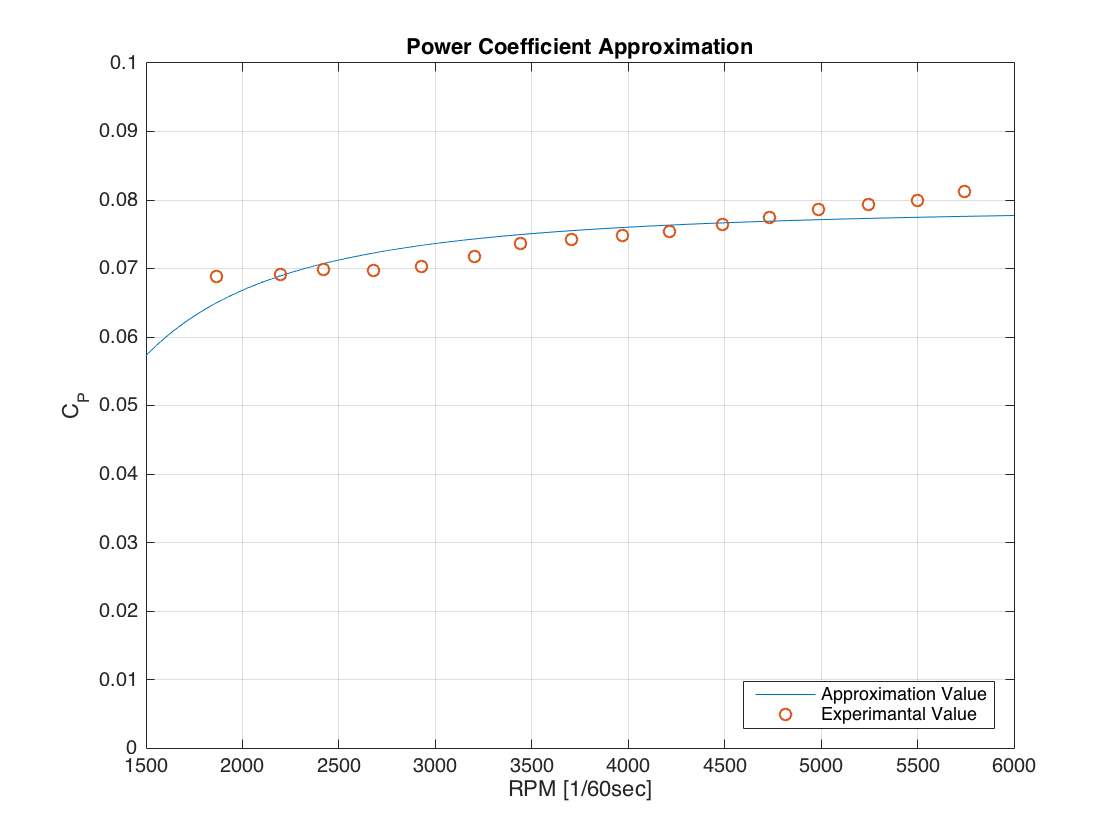
\includegraphics[width=0.8\textwidth]{graphics/Cp_fig.png}
    \caption{Comparison of experimental and approximated power coefficient}
    \label{fig:cp}
\end{figure}

To compute the model of thrust coefficient (\ref{eq:ct_approx}) and power coefficient (\ref{eq:cp_approx}), the experimental data of the propeller APC 10 \(\times\) 4.7 in the UIUC Propeller Database Vol.1 are used, and the method of least mean square error (LMSE) linear regression is applied in terms of \(1 \over {{n_i}^2}\) \cite{airfoil}. The approximated models of \(C_T (n_i)\) and \(C_P (n_i)\) are given as Equations (\ref{eq:ct}) and (\ref{eq:cp}), and the experimental data and the approximated models are compared in the Figures \ref{fig:ct}, \ref{fig:cp}. \\
\begin{equation}
\label{eq:ct}
\begin{aligned}
C_T ({n_i}) & = 0.1627 -73047 \times {1 \over {n_i}^2} \\
\end{aligned}
\end{equation}
\begin{equation}
\label{eq:cp}
\begin{aligned}
C_P ({n_i}) & = 0.0791 - 49112 \times {1 \over {n_i}^2} \\
\end{aligned}
\end{equation}
%%%%%%%%%%%%%%%%%%%%%%%%%%%%%%%%%%%%%%%%%%%%%%%%%%%%%%%%%%%%%%%%%%%%%%%%%%%%%%%%%%%%%%%%%%%%%%
\subsection{Motor Control}
In the quadrotor system, propellers are rotated by four brushless DC motors. In order to control DC motors, the method of pulse width modulation (PWM) is often used. In the PWM method, an average of constant-voltage pulsing signals actuates a motor \cite{audio}. Therefore, motor voltage is controllable by changing a pulse signal's width. Let \(d_{pwm}\) be duty cycle as, \\
\begin{equation}
\begin{aligned}
d_{pwm} = H f_{pwm} : \quad 0 \le d_{pwm} \le 1
\end{aligned}
\end{equation}
where \(H\) is signal width and \(f_{pwm}\) is the fixed frequency of signals. Then, the relation between motor voltage \(V_{mot}\) and duty cycle \(pwm\) is formalized as, \\
\begin{equation}
\label{eq:pwm_voltage}
\begin{aligned}
V_{mot} = d_{pwm} V_0
\end{aligned}
\end{equation}
where \(V_0\) is the constant voltage of signals.

The electric and dynamic models of a DC motor are given in terms of motor speed \(n\) and \(V_{mot}\) as,
\begin{equation}
\label{eq:motor_dynamics_01}
\begin{aligned}
V_{mot} & = 2 \pi k_{b} n + R i + L {{di}\over {dt}}\\
\end{aligned}
\end{equation}
\begin{equation}
\label{eq:motor_dynamics_02}
\begin{aligned}
k_m i & = 2 \pi k_f n + 2 \pi I_{mot} {{dn} \over {dt} } + M_R \text{sgn} (n)
\end{aligned}
\end{equation}
where \(k_{b} \), \(k_f\), \(k_m\) are the motor's torque constant, back electromotive force constant, and viscous damping coefficient, respectively. \(M_R\) is frictional torque, \(R\) is the motor's internal resistor, and \(L\) is the motor's internal inductance \cite{Mahfouz13}. \(I_{mot}\) is the total inertia of the motor and the propeller. Then, the above equation is written as the following second-order system with respect to motor speed \(n\). \\
\begin{equation}
\label{eq:motor_model_01}
\begin{aligned}
V_{mot} = 2 \pi \left( (k_b + {{R k_f}\over{k_m}} ) n + {1 \over {k_m}}( {R I_{mot}} + L k_f ) {{dn}\over{dt}} + {{L I_{mot}} \over {k_m} } {{d^2 n}\over{{dt}^2}}  \right) + R M_R \text{sgn} (n) : \quad n \neq 0\\
\end{aligned}
\end{equation}
Also, from Equation (\ref{eq:motor_dynamics_02}), there is a voltage threshold due to frictional torque so that a motor doesn't spin below the threshold. \\

Assuming motor speed changes smoothly so that the effect of internal resistor and inductance is small enough, Equation (\ref{eq:motor_model_01}) can be simplified as, \\
\begin{equation}
\label{eq:motor_model_02}
\begin{aligned}
V_{mot} \approx 2 \pi  (k_b + {{R k_f}\over{k_m}} ) n  + R M_R \text{sgn} (n)
\end{aligned}
\end{equation}
Define composite coefficients of the tangent \(\alpha\), and the intercept \(\beta\) as, 
\begin{equation}
\begin{aligned}
\alpha = {{k_m V_0} \over {2 \pi (k_b k_m + R k_f )}} 
\end{aligned}
\end{equation}
\begin{equation}
\begin{aligned}
\beta = {{k_m R M_R} \over {2 \pi (k_b k_m + R k_f )}} 
\end{aligned}
\end{equation}
Then, from Equations (\ref{eq:pwm_voltage}) and (\ref{eq:motor_model_02}), the relation between the motor speed \(n\) and the duty cycle \(d_{pwm}\) is written as the below equation.  \\
\begin{equation}
\label{eq:motor_curve_01}
\begin{aligned}
n \approx 
\begin{cases}
     \alpha d_{pwm}  - \beta \quad &  d_{threshold} \le d_{pwm} \le 1 \\
    0  \quad &   d_{pwm} \le  d_{threshold} \\
  \end{cases}
  \end{aligned}
\end{equation}

\begin{figure}
    \centering
    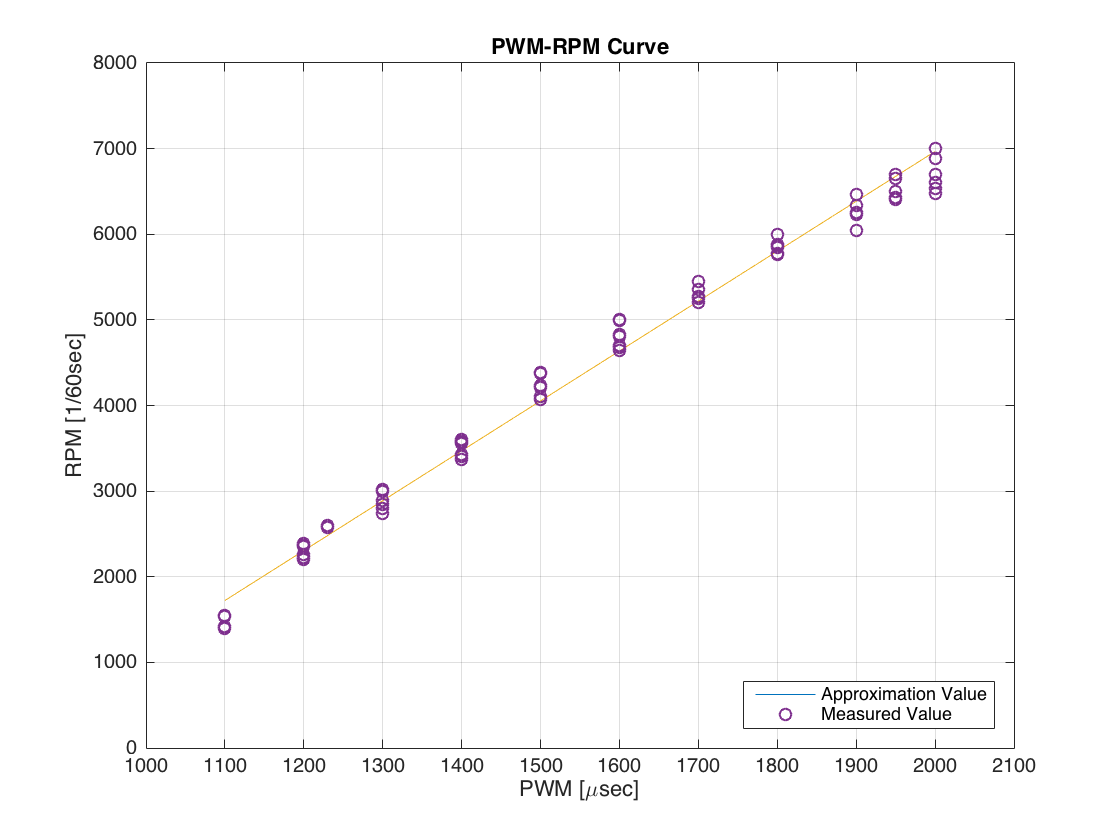
\includegraphics[width=0.8\textwidth]{graphics/pwm_rpm_curve.png}
    \caption{Change of RPM output corresponding to PWM command}
    \label{fig:pwm_rpm}
\end{figure}
If the characteristic information of the motors is available, the parameters \(\alpha\), \(\beta\) of the model of Equation (\ref{eq:motor_curve_01}) can be computed. However, there is no available information about the motor constants, it is necessary to calibrate the relation between PWM input and RPM output of a motor with a propeller. Therefore, the composite parameters of the gradient \(\alpha\) and the intercept \(\beta\) are calibrated by experiments. In the calibration, a reflective marker sticker is put on each propeller, and a tachometer measures rotation speed of the markers. PWM signal of voltage is controlled by an ESC, and the range of PWM command is set to be between 1000 \(\mu\)sec and 2000 \(\mu\)sec. The result of the experiment and the approximated model by the LMSE linear regression method are shown in Figure \ref{fig:pwm_rpm} and Equation (\ref{eq:motor_curve_02}).\\
\begin{equation}
\label{eq:motor_curve_02}
\begin{aligned}
n = 
\begin{cases}
     0.1716 \times d_{pwm}  - 803.4 \quad &  1100 \le d_{pwm} \le 2000 \\
    0  \quad &   \text{otherwise} \\
  \end{cases}
  \end{aligned}
\end{equation}


Since a brushless DC motor used in the quadrotor system does not have an encoder to measure its motor speed, open-loop control based on Equation (\ref{eq:motor_curve_02}) is applied to control motor speed. Also, PWM command is limited to be between 1230 \(\mu\)sec and 1950 \(\mu\)sec to prevent inappropriate performance.
